% 
% chapter5.tex
% ThesisISEL
% 
% Created by Serge Lage on 2019/07/30.
%
% ================
% = Introduction =
% ================
\chapter{Joined Fishery Analysis}
\label{cha:server}
This chapter explains the approach used to reach the second goal of this work. 

In Section 4.1 we implement the methodology learn in Section \ref{sub:crisp_dm} to approach  goal 2.



\section{Implementation of CRISP-DM} % (fold)
\label{sub:implementation}

\subsection{Business Understanding} % (fold)
\label{sub:business_understanding}

In the fishing sector, vessels operating in the various fishing techniques must be licensed.
A common problem is that there is a likelihood that vessels will be fishing for which they are not licensed. The objective is to obtain a predictive model, capable of receiving VMS data and proceed to its classification in order to predict which type of fishing is being carried out by the vessel. In this way, it will be possible to ascertain whether or not a given vessel is carrying out a legal fishing activity, that is, according to the license it has.



% section business_understanding (end)


\subsection{Data Understanding} % (fold)
\label{sub:data_understanding}

To answer this goal, the data used as input are the same VMS Records as used in Chapter 3, initially presented in Chapter 1, Section 1.3.1 and VMS Vessels presented in Chapter 1, Section 1.3.2. The output variable is nominal whose categories correspond to the labels of the different fishing licenses.

% section data_understanding (end)



\subsection{Data Preparation} % (fold)
\label{sub:data_preparation}
To use data mining models, a first step is to build a dataset with all the data needed to feed the models. So, it was created a dataset from VMS Vessels and VMS Records to end with Table \ref{table:vms_dataset}. 
The correlation between the license and the HP data (vessel power), Loa (Boat length), Gt (vessel weight) are quite significant. This is expected as different fishing activities require specific types of vessels. This does not mean that the type of vessel is only capable of entering a type of fishing activity.
For these reasons, we will not use these variables in the model so as not to create a problem with bias.

\begin {table}[H]
\caption {VMS Dataset}
\begin{center}
\begin{tabular}{c|c|c|c}
\textbf{Name } & \textbf{Description} & \textbf{From} & \textbf{Why} \\
\hline
ID & Key & Native & Identify the row \\
VesselID & Vessel Identifier & VMS Records & Identify the vessel \\
UTC & Date Time & VMS Records &Identify the time of the entry\\
LAT & Latitude & VMS Records & Discriminated by fishing areas\\
LON & Longitude & VMS Records & Discriminated by fishing areas\\
COG & Direction & VMS Records & Course Over Ground\\
SOG & Velocity & VMS Records & Discriminated by fishing velocity\\
%LOA & Length Overall & VMS Vessels & Discriminated by vessel type\\
%GT & Gross Tonnage & VMS Vessels & Discriminated by vessel type\\
%HP &Vessel Power & VMS Vessels & Discriminated by vessel type\\
License & Vessel's Linceses & VMS Vessels & Objective
\label{table:vms_dataset}
\end{tabular}
\end{center}
\end {table}



When analyzing the speed distribution by license, we can observe in Figure \ref{fig:sogall} that there is no obvious difference between licenses. For example the value 1 of SOG can be assigned to any license.

\begin{figure}[H]
\centering
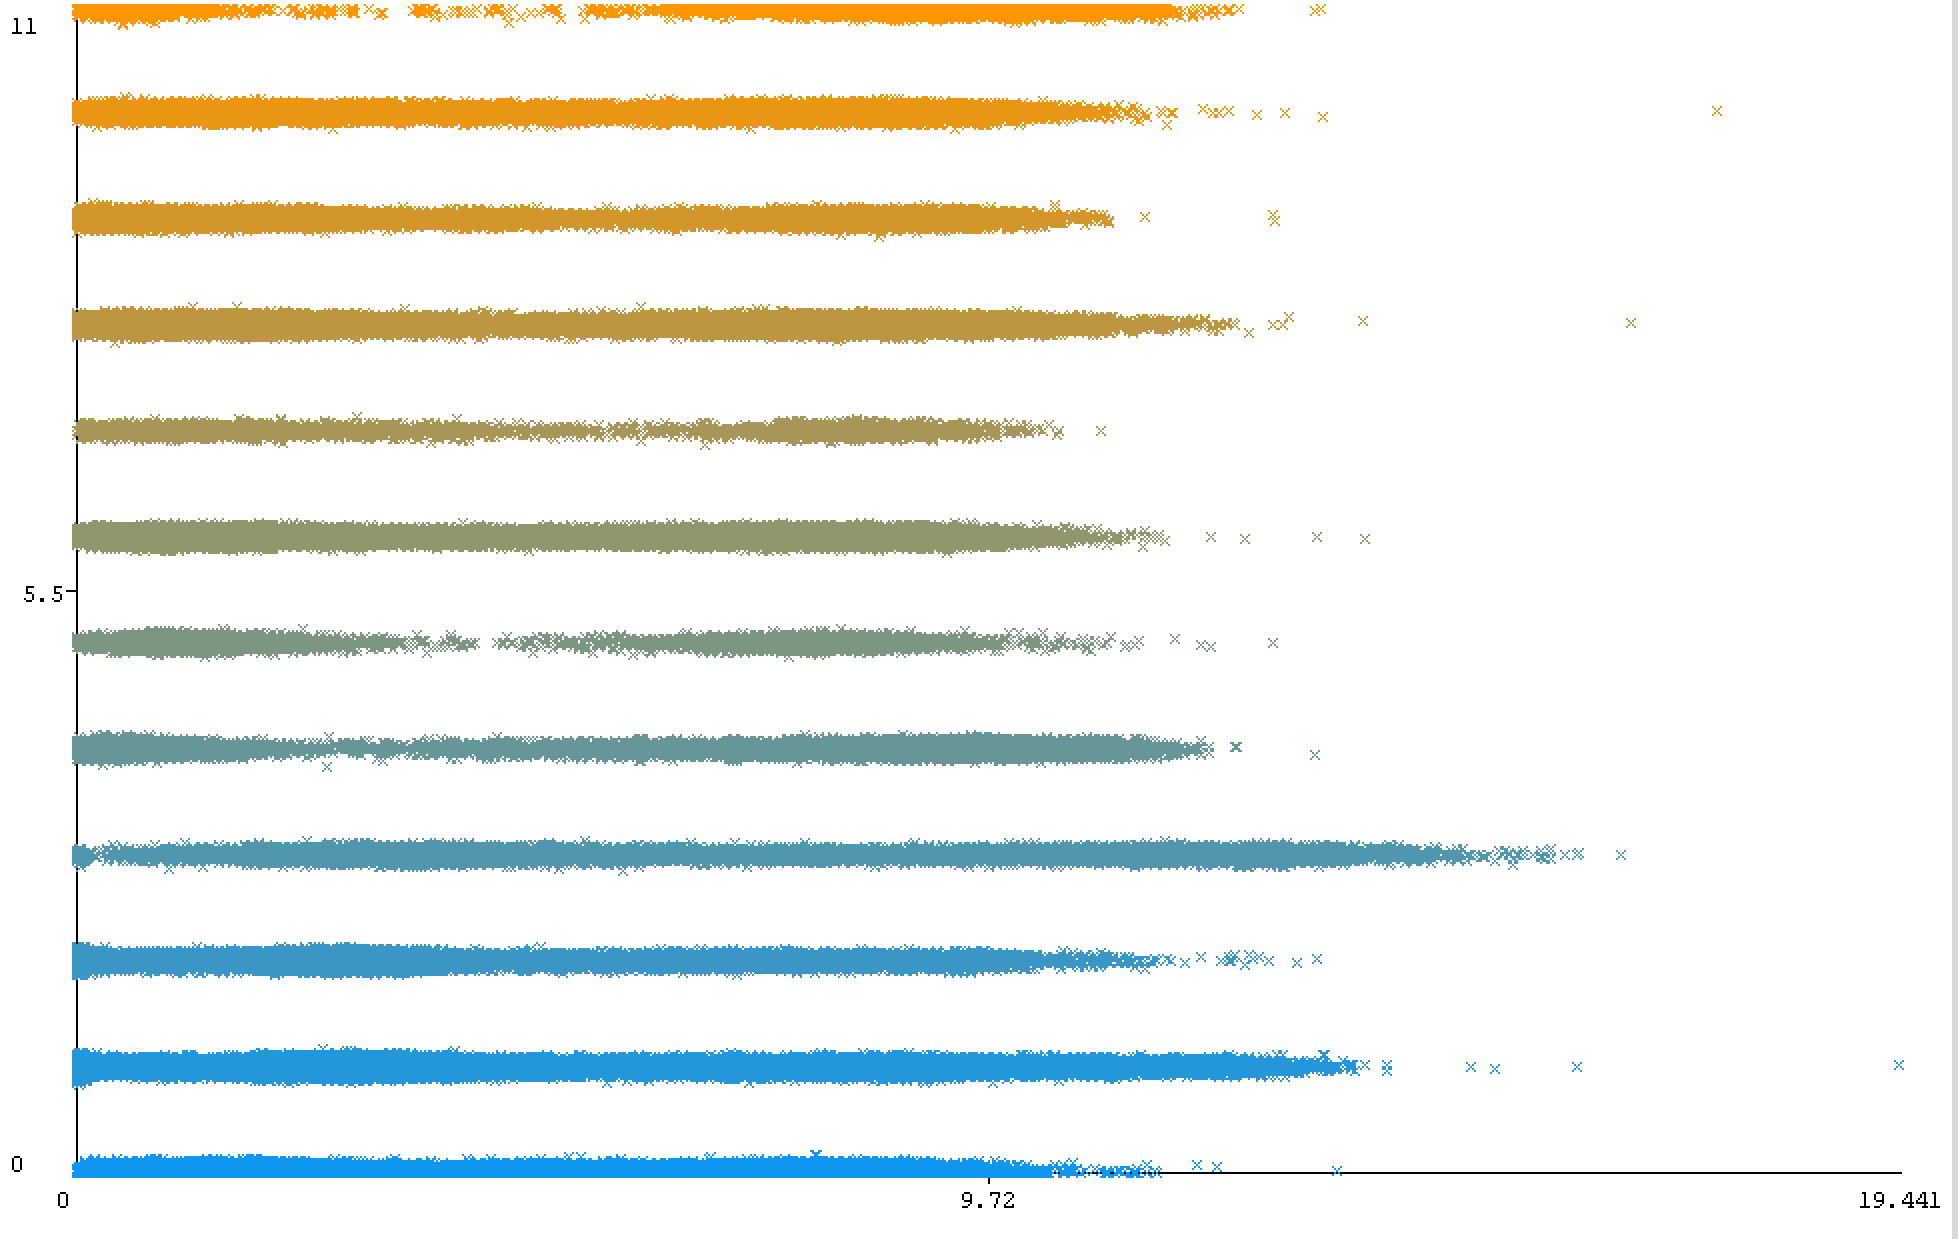
\includegraphics[width=0.5\linewidth]{Chapters/img/sog_all_2.png}
\caption{SOG per license}
\label{fig:sogall}
\end{figure}

To try to help the predictive model to have good results, some pre-processing is necessary. A simple and effective way is to group data by vessel and activity day. Then apply the SFA to the data to have, per day, per vessel, the minimum fishing speed, maximum fishing speed and also remove the average speed.
With these three variables, it is possible to better distinguish the behavior of vessels by license through speed.

\begin{figure}
\centering
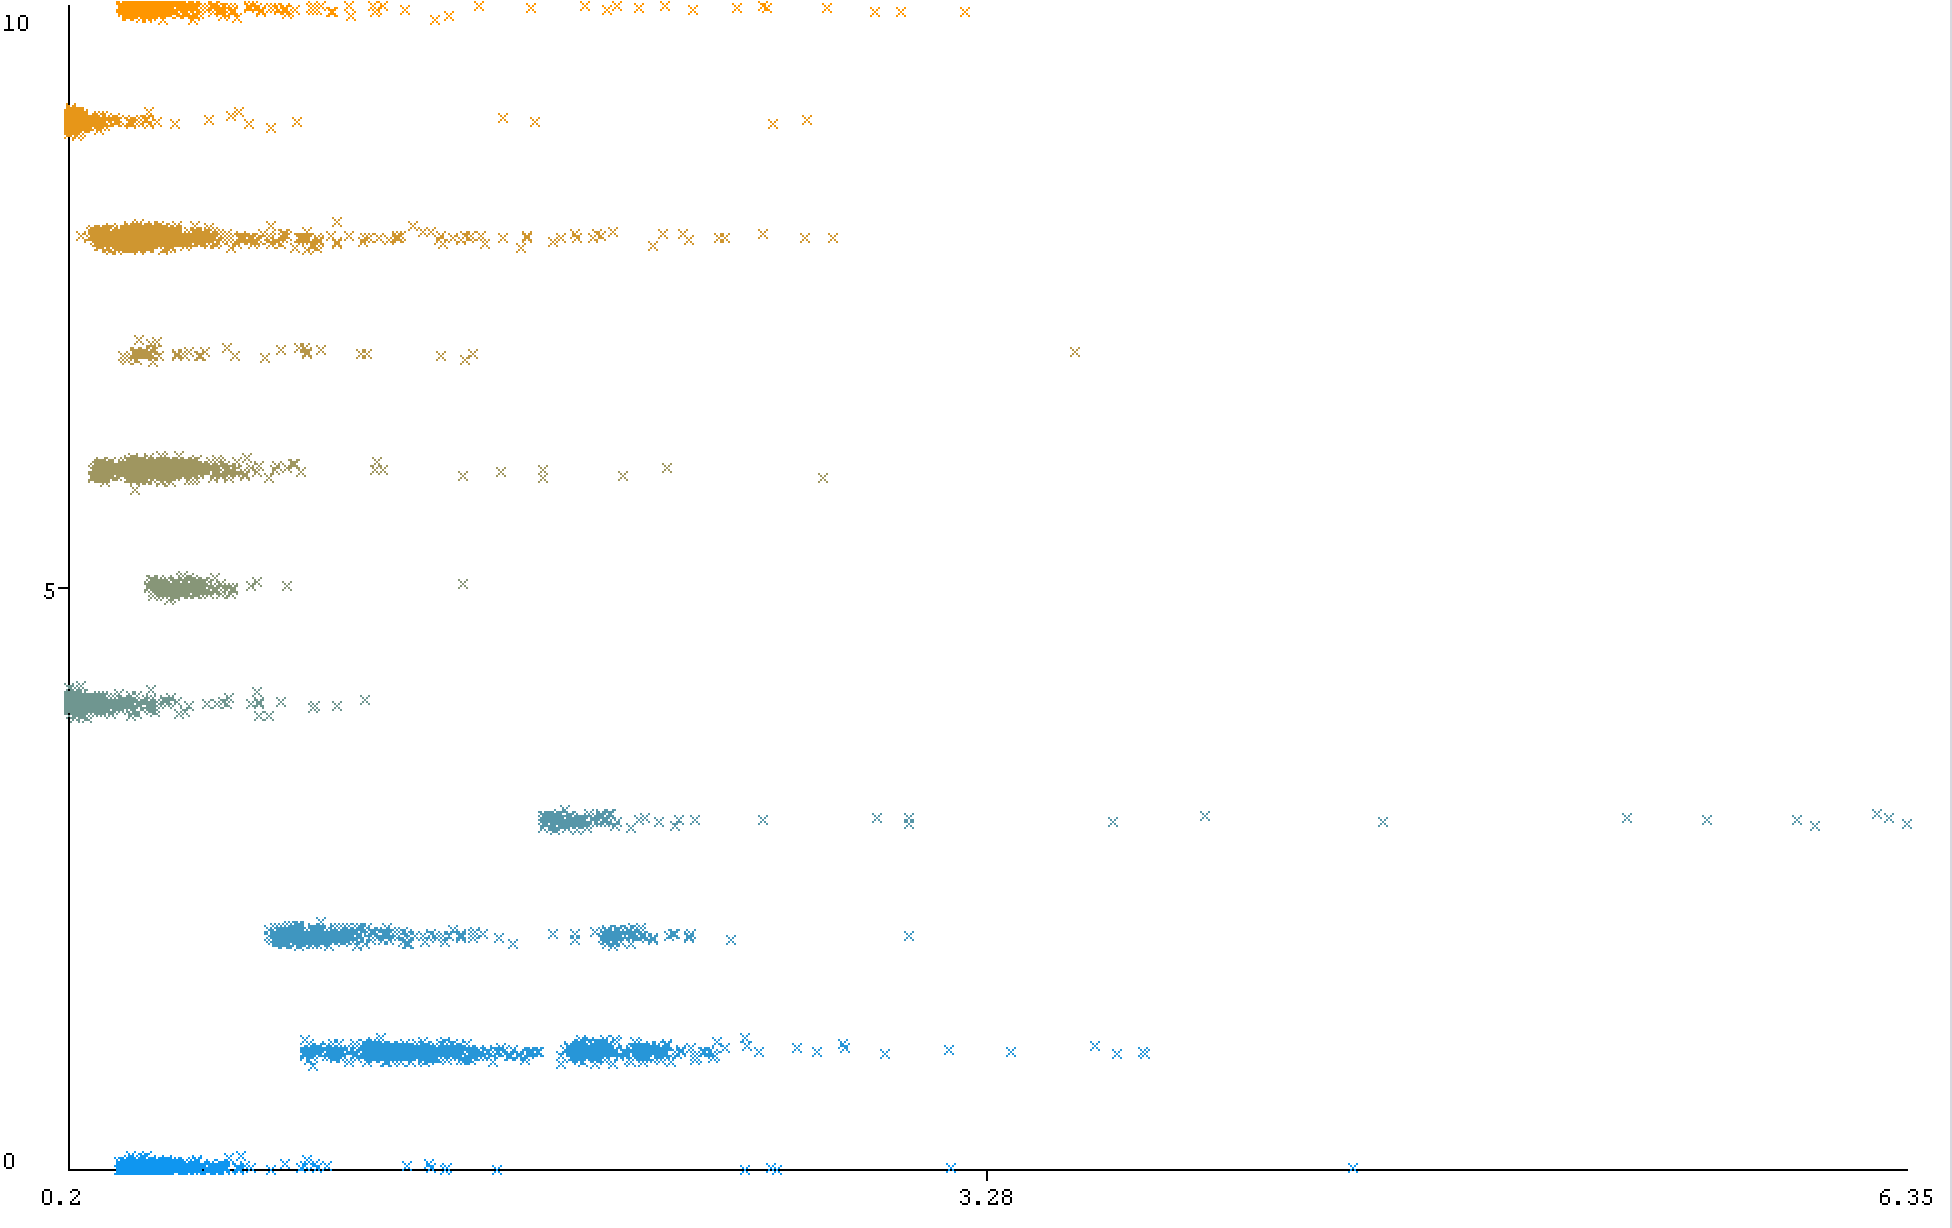
\includegraphics[width=0.5\linewidth]{Chapters/img/sog_min_2.png}
\caption{SOG minimum per license}
\label{fig:sogminall}
\end{figure}
\begin{figure}
\centering
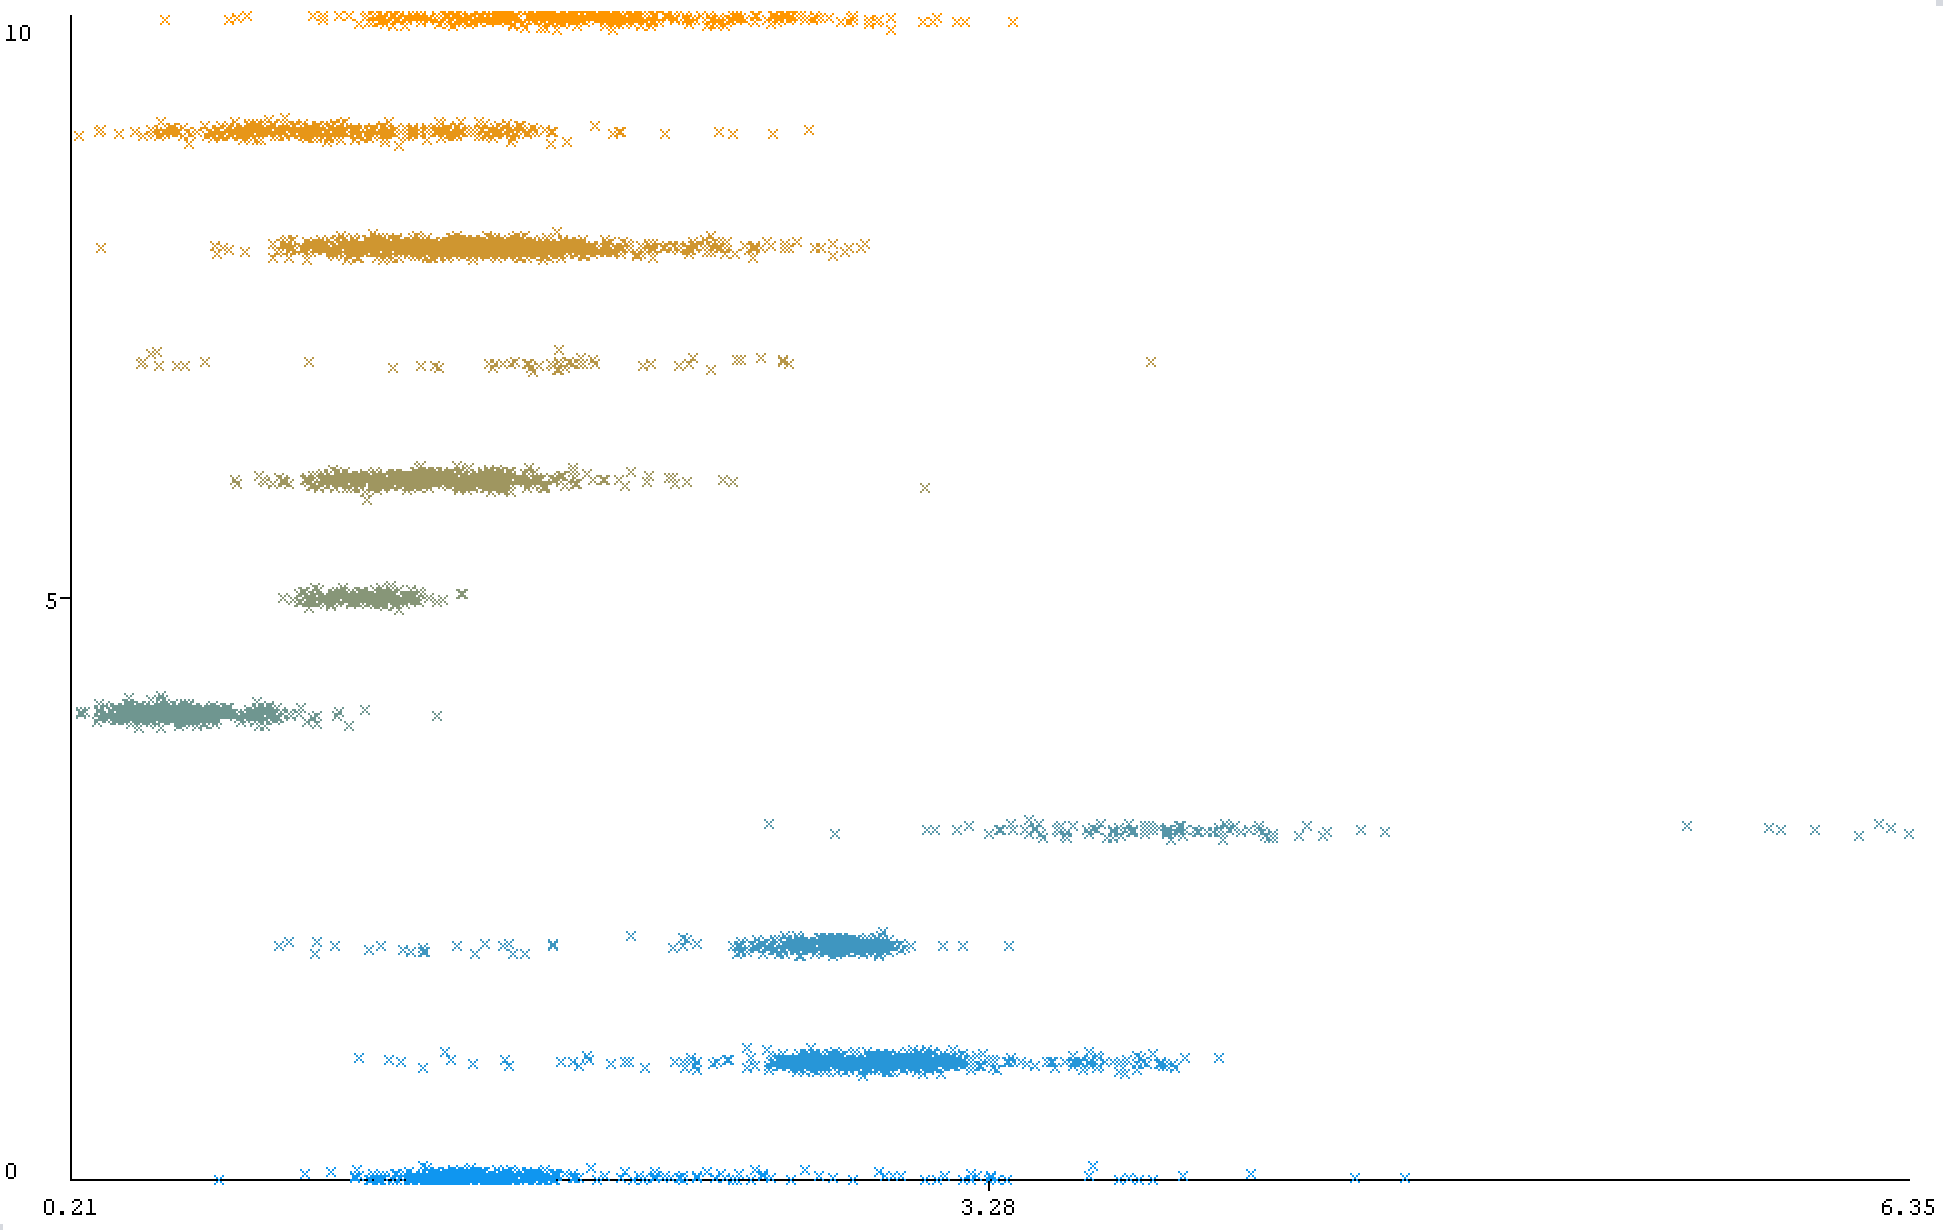
\includegraphics[width=0.5\linewidth]{Chapters/img/sog_avg_2.png}
\caption{SOG average per license}
\label{fig:sogavgall}
\end{figure}
\begin{figure}
\centering
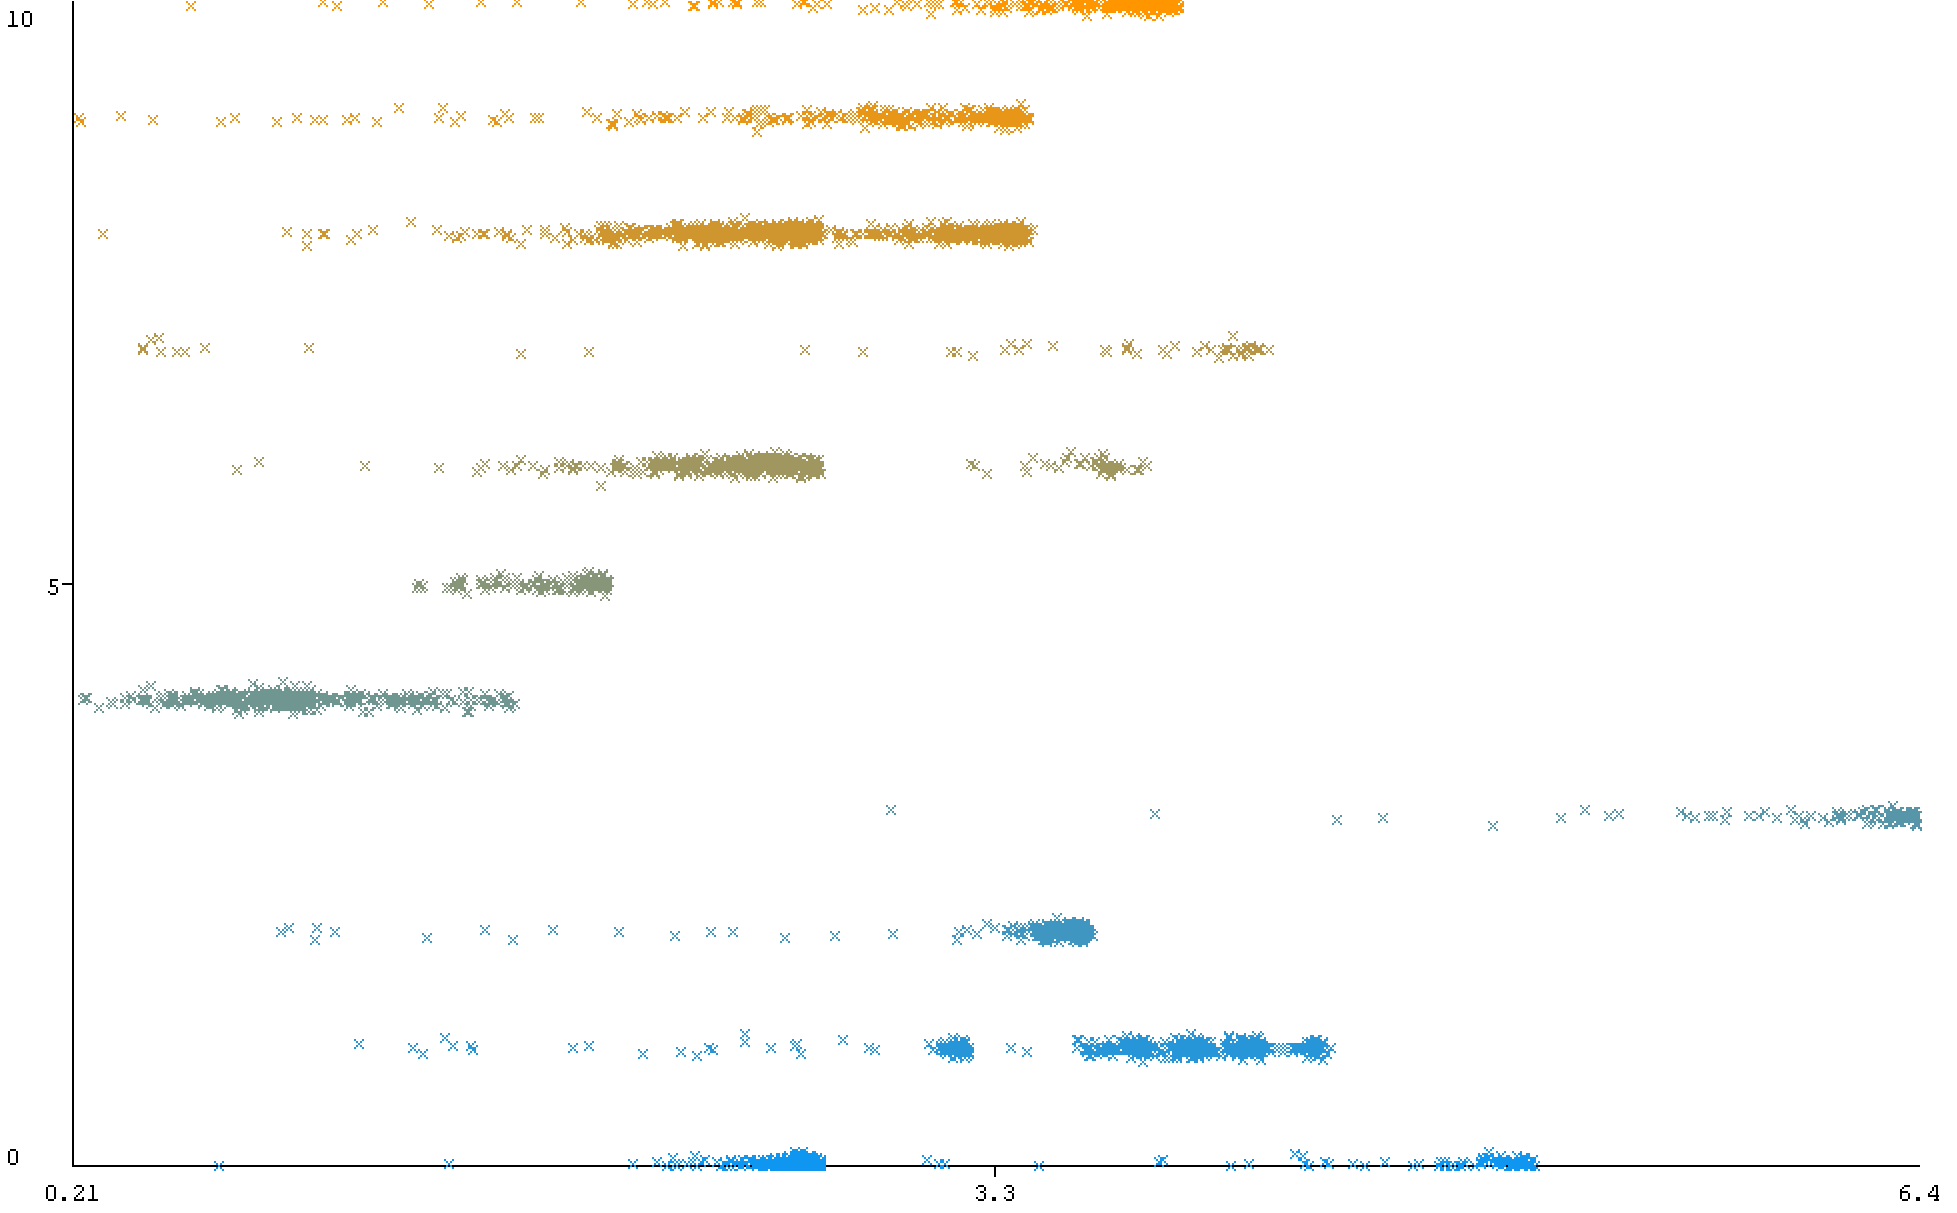
\includegraphics[width=0.5\linewidth]{Chapters/img/sog_max_2.png}
\caption{SOG maximum per license}
\label{fig:sogmaxall}
\end{figure}


The method used to transform the data consists of the following steps:
\begin{itemize}
\item Create a dataset in which data are grouped per day, per vessel.
\item Use DSALib to get the minimum and maximum speeds of fishing per vessel. From this data, apply a filter to obtain observations for which the velocity varies between its minimum and maximum value.

\end{itemize}


Regarding location data, clustering techniques to discretize the data were used.
First, the best number of clusters is determined. For that, we used the same technique as in Section 4.3, resulting the Figure \ref{fig:elbow_method_server}. The data used was the dataset filtered, so we have only the positions of fishing. The chosen number of clusters was 6.

\begin{figure}[H]
\centering
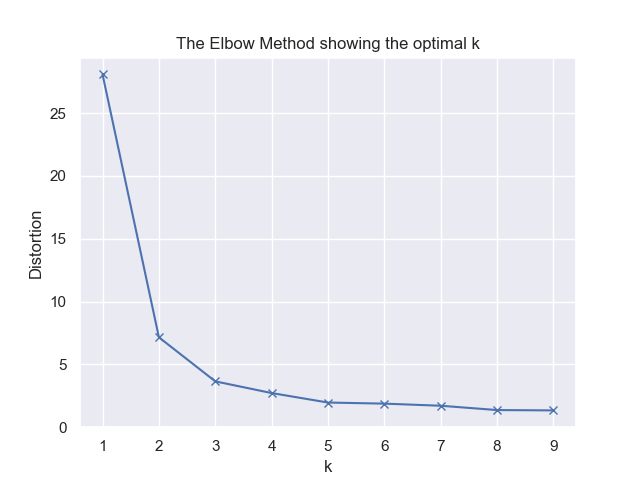
\includegraphics[width=0.8\linewidth]{Chapters/img/elbow_method_server.png}
\caption{The elbow method showing the optimal k}
\label{fig:elbow_method_server}
\end{figure}
Now, is possible to create data mining models based on the location and on the velocity patterns. 


% section data_preparation (end)
\newpage
\subsection{Modeling} % (fold)
\label{sub:modeling}
In order to classify a new type of license using VMS data, several data mining algorithms were tested, which we now list:
\begin{itemize}
\item \textbf{ KMeans-} This model was used to organize GPS data in clusters to improve the result of the data mining algorithms. The operating mode of this algorithm has already been covered in the Section \ref{sub:kmeans}.
The implementation used was KMeans from the sklearn library \cite{WEBSITE:scikit}.

\item \textbf{ Decision Trees- } This model was used to classify the fishing license from VMS data. The operating mode of this algorithm has already been covered in the Section \ref{subsub:decision_trees}. The implementation used was DecisionTreeClassifier from the sklearn library.


\item \textbf{ Random Forests- } This model was used to classify the fishing license from VMS data. The operating mode of this algorithm has already been covered in the Section \ref{subsub:random_forests}. The implementation used was RandomForestClassifier from the sklearn library.


\item \textbf{Neural Network- } This model was used to classify the fishing license from VMS data. The operating mode of this algorithm has already been covered in the Section \ref{subsub:neural_network}. The implementation used was MLPClassifier from the sklearn library.

\item \textbf{Support Vector Machine- } This model was used to classify the fishing license from VMS data. The operating mode of this algorithm has already been covered in the Section \ref {subsub:svm}. The implementation used was SVC from the sklearn library.
\end{itemize}


% section modeling (end)

\subsection{Evaluation} % (fold)
\label{sub:evaluation}
Cross \textendash validation \cite{CrossValidatory} provides a simple and effective method for both model selection and performance evaluation, widely employed by the machine learning community. Under k \textendash fold cross \textendash validation, the data are randomly partitioned to form k disjoint subsets of approximately equal size. In the ith fold of the cross-validation procedure, the ith subset is used to estimate the generalization performance of a model trained on the remaining k \textendash 1 subset. The average of the generalization performance observed overall k folds provides an estimate (with a slightly pessimistic bias) of the generalization performance of a model trained on the entire sample.
To evaluate these models a 10-fold, k=10, cross - validation was performed. \\
To evaluate the classification results customized with the different algorithms, a confusion matrix, as described in table \ref{table:cm_ex} created and interpreted according ours goals. 

\begin {table}[H]
\caption {Confusion matrix}
\begin{center}
\begin{tabular}{cc|cc}
\multicolumn{1}{c}{} &\multicolumn{1}{c}{} &\multicolumn{2}{c}{Predicted} \\ 
\multicolumn{1}{c}{} & 
\multicolumn{1}{c|}{} & 
\multicolumn{1}{c}{Positive} & 
\multicolumn{1}{c}{Negative} \\ \hline
\multirow[c]{2}{*}{\rotatebox[origin=tr]{90}{Actual}}
& Positive & True Positive(TP) & False Negative(FN) \\[1.5ex]
& Negative & False Positive(FP) & True Negative(TN) \\ \hline
\label{table:cm_ex}
\end{tabular}
\end{center}
\end {table}

In addition, the following performance indicators were used:\\
Precision, also called as positive predictive value attempts to identify what proportion of positive identifications was actually correct, is given by \ref{eq:precision}. \\
\begin{equation}
\sum_{n=0}^{k-1}\frac{tp}{tp+fp} 
\label{eq:precision}
\end{equation}

Recall, also called as sensitivity attempts to identify what proportion of actual positives was identified correctly \ref{eq:recall}. \\
\begin{equation}
\sum_{n=0}^{k-1}\frac{tp}{tp+fn} 
\label{eq:recall}
\end{equation}

%Accuracy = \( \sqrt{precision} ^ 2\) = accuracy of the precision result.\\
%Precision = \(\sum_{n=0}^{k-1}\frac{tp}{tp+fp} \) = precision of the model.\\
%Recall = \(\sum_{n=0}^{k-1}\frac{tp}{tp+fn} \) = recall of the model.\\



A confusion matrix \cite{CMPatil} illustrates the accuracy of the solution to a classification problem. Given n classes, a confusion matrix has general element C\textsubscript{i,j} corresponding to the number of tuples from D that were assigned to class C\textsubscript{i,j}, but where the correct class is C\textsubscript{i}.
The best solution will have only zero values outside the diagonal.
A confusion matrix contains information about actual and predicted classifications done by a classification system. The performance of such systems is commonly evaluated using the data in the matrix. Table \ref{table:cm_ex} shows the confusion matrix for a two-class classifier. 

For the purpose of this work, the classes corresponding to the different types of licenses are: 

0 Armadilhas / De abrigo / Alcatruzes \\
1 Arrasto / De fundo de portas \\
2 Arrasto / De fundo de portas / Crustáceos\\
3 Arrasto / Pelágico / Com portas\\
4 Cerco / para bordo / Tipo americano\\
5 Emalhar de 1 pano / De deriva / Grandes Pelágicos\\
6 Emalhar de 1 pano / De fundo\\
7 Pesca à linha / Cana e linha de mão\\
8 Pesca à linha / Palangre de fundo / Espécies demersais\\
9 Pesca à linha / Palangre de Fundo + Cana e linha de mão\\
10 Pesca à linha / Palangre de superfície / Grandes Migradores



The model's test results are:

\begin{itemize}
\item \textbf{ Decision Trees: }

We can observe in Table \ref{table:cross_val_dt} the usage of velocity parameters (SogMin, SogAVG, and SogMax) and location (clustering result of K-Means) having the best result. The algorithm with the best result is Entropy(C4.5), with a precision of 0.8142 and an recall of 0.8142. In Figure \ref{table:cross_val_dt} the confusion matrix shows that only the classes 0 and 7 have a low prediction rate. The max depth of the trees was tested as 200, 300, and 400, with 300 giving the best results.


\begin {table}[H]
\caption {Cross-Validation results for Decision Trees models}
\begin{center}
\begin{tabular}{c|c|c|c|c}
\multicolumn{1}{c|}{\textbf{Splitting criteria } } &\multicolumn{2}{c|}{\textbf{ Velocity and locations}}& \multicolumn{2}{c}{\textbf{ Velocity}}\\
&Precision & Recall & Precision & Recall \\
\hline
Gini & 0.8047& 0.8047&0.7479&0.7479\\
Entropy& 0.8142& 0.8142&0.7659&0.7659
\label{table:cross_val_dt}
\end{tabular}
\end{center}
\end {table}

\begin{figure}[H]
\centering
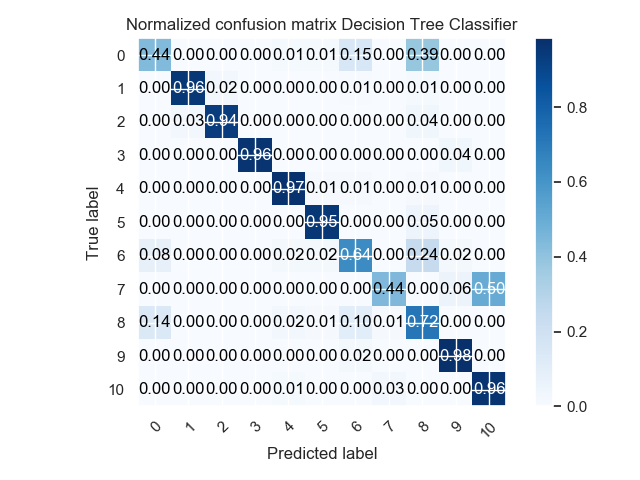
\includegraphics[width=0.8\linewidth]{Chapters/img/CM_DT.png}
\caption{Confusion Matrix for Decision Tree using Entropy splitting criterion(C4.5)}
\label{fig:cm_dt}
\end{figure}


\newpage
\item \textbf{ Random Forest: }
Concerning Random forest use, the model was trained again considering Giny impurity and Entropy Information Gain as splitting criteria. 
The results obtained in Decision Trees are confirmed in this model, being the usage of Entropy criteria the best results ( better precision). 
So the results mentioned in this document for Random Forest models are using Entropy(C4.5) as the algorithm to measure the quality of a split. The max depth of the trees was tested with the values of 200, 300, and 400, being the best results attained with the max depth value of 300. Table \ref{table:cross_val_rf}, describes the cross-validation results obtained with the Random Forest model, for 200 number of estimators. 
In Figure \ref{table:cross_val_rf} is shown the confusion matrix corresponding to the Random forest classifier. The results are satisfactory given that only the classes 0 and 7 have a lower correct prediction rate.

\begin {table}[H]
\caption {Cross-Validation results for Random Forest models}
\begin{center}
\begin{tabular}{c|c|c|c|c}
\multicolumn{1}{c|}{\textbf{No. of estimators } } &\multicolumn{2}{c|}{\textbf{ Velocity and locations}}& \multicolumn{2}{c}{\textbf{ Velocity}}\\
&Precision & Recall & Precision & Recall \\
\hline
50 &0.8389&0.8389 &0.8 &0.8\\
100 &0.8398&0.8398 &0.7896 &0.7896\\
200 &0.8474&0.8474 &0.7953 &0.7953 \\
300 &0.8445&0.8445 &0.7943 &0.7943 
\label{table:cross_val_rf}
\end{tabular}
\end{center}
\end {table}


\begin{figure}[h]
\centering
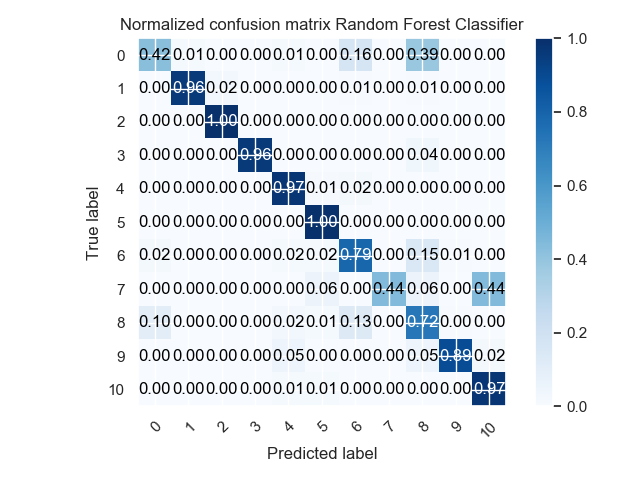
\includegraphics[width=0.8\linewidth]{Chapters/img/CM_RF.png}
\caption{Confusion Matrix for Random Forest using 200 estimators}
\label{fig:cm_rf}
\end{figure}


\newpage
\item \textbf{Neural Network: }\\
For these models, it was trained in various configurations of hidden layers. It was used from 1 to 8 hidden layers with 11, 100, 250, 500, and 750 neurons. Some of the results are in Table \ref{table:cross_val_nn}. The best result, as we can observe in Table \ref{table:cross_val_nn} corresponds to the case with five layers with 500 neurons for which the confusion matrix is presented in Figure \ref{fig:cm_nn}.
For some models, it was used the Adam solver and BFGS, but with BFGS having better results. So all reported results are using BFGS solver.
As in Decision Trees models, the usage of locations has a good impact on the results of the Neural Network models.


\begin {table}[H]
\caption {Cross-Validation results for Neural Network models}
\begin{center}
\begin{tabular}{c|c|c|c|c}
\multicolumn{1}{c|}{\textbf{Hidden Layers } } &\multicolumn{2}{c|}{\textbf{ Velocity and locations}}& \multicolumn{2}{c}{\textbf{ Velocity}}\\
&Precision & Recall & Precision & Recall \\
\hline
11 &0.7175&0.7175&0.6730 &0.6730\\
100 &0.7507&0.7507&0.70426 &0.7043\\
4 500 &0.7536&0.7536&0.7715& 0.7715\\
5 500 &0.7479&0.7479&0.7659& 0.7659\\
6 500 &0.7867&0.7867&0.7583&0.7583
\label{table:cross_val_nn}
\end{tabular}
\end{center}
\end {table}


\begin{figure}[h]
\centering
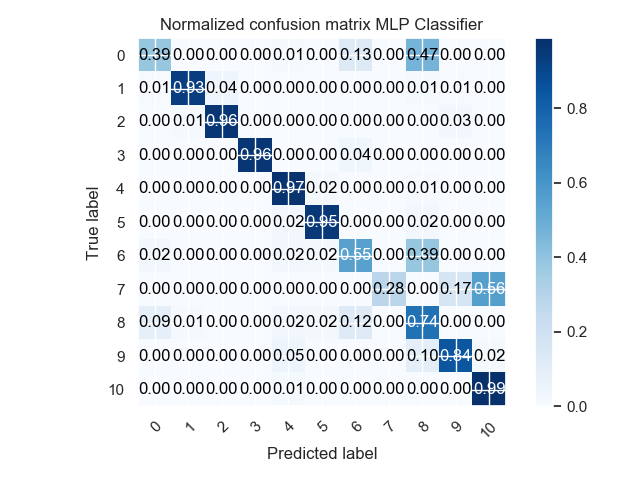
\includegraphics[width=0.8\linewidth]{Chapters/img/CM_NN.png}
\caption{Confusion Matrix for Neural Network using 5x500 hidden layers}
\label{fig:cm_nn}
\end{figure}


\newpage
\item \textbf{Support Vector Machine: }\\
For the built of support vector machine models, it was used the type of kernel of Polynomial, RBF, and linear. With the best result as we can observe in Table \ref{table:cross_val_svm} is the Polynomial, with its confusion matrix represented in Figure \ref{fig:cm_cvm}. 



\begin {table}[H]
\caption {Cross-Validation results for Support Vector Machine models}
\begin{center}
\begin{tabular}{c|c|c|c|c}
\multicolumn{1}{c|}{\textbf{Kernel coefficient } } &\multicolumn{2}{c|}{\textbf{ Velocity and locations}}& \multicolumn{2}{c}{\textbf{ Velocity}}\\
&Precision & Recall & Precision & Recall \\
\hline
Polynomial &0.7422&0.7422&0.672&0.672\\
RBF &0.7374&0.7374&0.6986&0.6986\\
Linear &0.6569&0.6568&0.545&0.545
\label{table:cross_val_svm}
\end{tabular}
\end{center}
\end {table}

\end{itemize}

\begin{figure}[h]
\centering
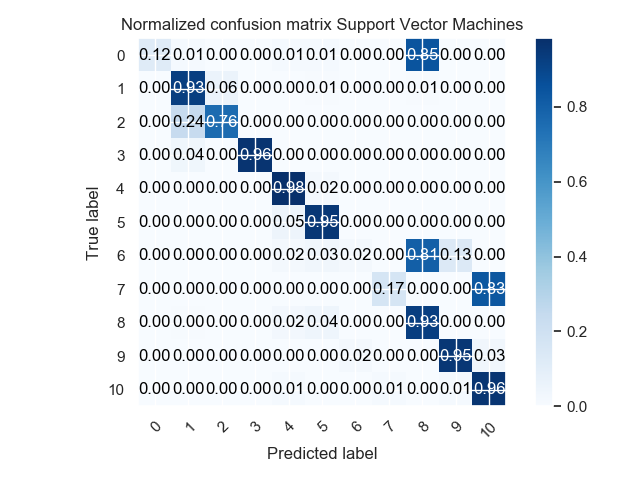
\includegraphics[width=0.8\linewidth]{Chapters/img/CM_SVM.png}
\caption{Confusion Matrix for Support Vector Machine using Polynomial kernel coefficient}
\label{fig:cm_cvm}
\end{figure}


\newpage


The model with the best result corresponds to the use of a random forest method, with the configuration of 200 estimators. For this model was obtained a precision of 84.74\%.
With this, we can determine that it is possible to create a good model to classify the VMS data as the fishing license. \\
As seen in Figure \ref{fig:cm_rf}, the classes 0 and 7 have a low true positive rate. The usage of more data and data that are certified that the VMS data of a vessel is only for the purpose of the fishing license can improve the precision of the model.


%Determine Next Steps
%List of Possible Actions
%Decision

% section evaluation (end)


\subsection{Deployment} % (fold)
\label{sub:deployment}

%Plan Deployment Deployment Plan
To use the trained model, we separated JFA into 4 steps:
\begin{enumerate}
\item \textbf{ Receive VMS data and register in a BD.} JFA needs to be able to receive VMS data so it can classify it, but it is also important to persist the data in a way that we can update the model with more recent data. 

\item \textbf{Pre process the data.} If SFA is installed in the blue box that is filling the VMS data, the data entries can be already classified as fishing or not fishing. If not, JFA needs to collect data and run its local SFA for each vessel that does not have SFA. If the data is received in one time when the vessel arrives at the port, convert all the data received, as explained in Subsection \ref{sub:data_preparation}. If the blue box is broadcasting data when the vessel is on activity, we can classify the data as fishing or not (if SFA not installed in the blue box) and have a subsystem that detects when a vessel fails to send data or have stopped fishing for more than some defined time. This will allow time as the competent authorities will prepare an inspection as marked vessels even before reaching the port.

\item \textbf{Use the model to classify.} With the data obtained in the last step, use the model tested chosen in Subsection \ref{sub:evaluation}.

\item \textbf{Validate vessel license comparison, send an alert.} Compare the class attributed by the model with the license of the vessel and, if different, register and send a message to the designated authority.

\end{enumerate}

%Plan Monitoring and Maintenance
To keep the model up to date, it is essential to train a new model with recent data from time to time. If possible, to know that data is verified by a competent authority, when training the model gives more relevance to this verified data. This is important because the train data that is not verified can be given by vessels that are not respecting their fishing license and this way corrupting the model.


% section deployment (end)

% chapter server (end)





